\documentclass[12pt]{article}
\usepackage{graphicx}
\usepackage{float}
%% FONTS
%% To get the default sans serif font in latex, uncomment following line:
 \renewcommand*\familydefault{\sfdefault}
%%
%% to get Arial font as the sans serif font, uncomment following line:
%% \renewcommand{\sfdefault}{phv} % phv is the Arial font
%%
%% to get Helvetica font as the sans serif font, uncomment following line:
% \usepackage{helvet}
\usepackage[small,bf,up]{caption}
\renewcommand{\captionfont}{\footnotesize}
\usepackage[left=1in,right=1in,top=1in,bottom=1in]{geometry}
\usepackage{graphics,epsfig,graphicx,float,subfigure,color}
\usepackage{amsmath,amssymb,amsbsy,amsfonts,amsthm}
\usepackage{url}
\usepackage{boxedminipage}
\usepackage[sf,bf,tiny]{titlesec}
 \usepackage[plainpages=false, colorlinks=true,
   citecolor=blue, filecolor=blue, linkcolor=blue,
   urlcolor=blue]{hyperref}
\usepackage{enumitem}
\usepackage{verbatim}
\usepackage{tikz,pgfplots}

\newcommand{\todo}[1]{\textcolor{red}{#1}}
% see documentation for titlesec package
% \titleformat{\section}{\large \sffamily \bfseries}
\titlelabel{\thetitle.\,\,\,}

\newcommand{\bs}{\boldsymbol}
\newcommand{\alert}[1]{\textcolor{red}{#1}}
\setlength{\emergencystretch}{20pt}
\title{Spring 2022: Advanced Topics in Numerical Analysis: \\
High Performance Computing\\Homework 3 \\ \hyperref[Github]{https://github.com/anmolsinghal/HPCHW3}} 
\author{Submitted by: Anmol Singhal \\ as15151@nyu.edu}

\date{}
\hypersetup{
    colorlinks=true,
    linkcolor=blue,
    filecolor=magenta,      
    urlcolor=cyan,
}
\begin{document}


\maketitle
% ****************************
\begin{enumerate}
% --------------------------
\item {\bf Pitch your final project.} \\
  Submitted previously

  \item {\bf Approximating Special Functions Using Taylor Series \& Vectorization.} \\
  fast-sin.cpp has the \texttt{sin4\_vec()} function improved to provide higher accuracy of upto 12 decimal places. \\
  Also added logic to calculate value of sin for any input using taylor series approximation. To use the function, need to change the range of input to the desired range.
   
    % ***************************
  \item {\bf Parallel Scan in OpenMP.} 
  Results in image provided. Tests are run on CIMS server and the speedup is observed till upto 8 threads after which performance tapers off.

  \begin{figure}[H]
    \caption{Results of speed up of fast-sin as welll as omp-scan}
    \centering
    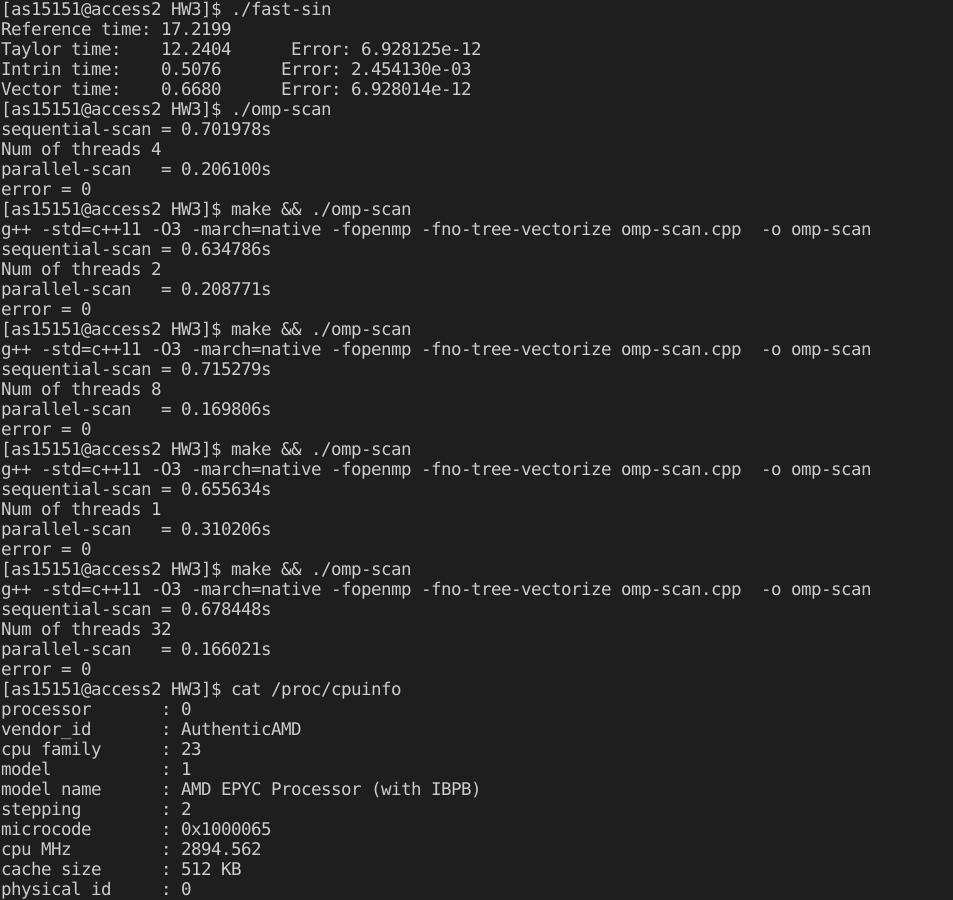
\includegraphics[width=\textwidth]{results.png}
    \end{figure}
\end{enumerate}


\end{document}
